\begin{section}{SC}{RADAMESH: Cosmological Radiative Transfer for Adaptive Mesh\\
    \hspace*{4cm} Refinement Simulations}{(Prof. Sebastiano Cantalupo)}
  \begin{minipage}[l]{\textwidth}

    {\small RADAMESH is a three-dimensional radiative transfer (RT) code, based
      on a ray-tracing, photon-conserving and adaptive (in space and time)
      scheme. It uses a novel Monte Carlo approach to sample the radiation field
      within the computational domain on a ”cell-by-cell” basis. Thanks to this
      algorithm, the computational efforts can be focused where needed most,
      i.e. within the Ionization-fronts (I-fronts). This results in an increased
      accuracy level and a huge gain in computational speed with respect to a
      ”classical” Monte Carlo RT, especially when combined with an Adaptive Mesh
      Refinement (AMR) scheme. RADAMESH is able to adaptively refine the
      computational mesh in correspondence of the I-fronts, allowing to fully
      resolve them within large, cosmological boxes. The propagation of ionizing
      radiation is followed from an arbitrary number of sources and from the
      recombination radiation produced by H and He. The chemical state of six
      species (HI, HII, HeI, HeII, HeIII, e) and gas temperatures are computed
      with a time-dependent, non-equilibrium chemistry solver. Using our AMR
      scheme, we find that properly resolving the I-front of a bright quasar
      during Reionization produces a large increase of the predicted gas
      temperature within the whole HII region.}
  \end{minipage}

  \vspace{0.5cm}

  \begin{minipage}{\linewidth}
    \begin{center}
      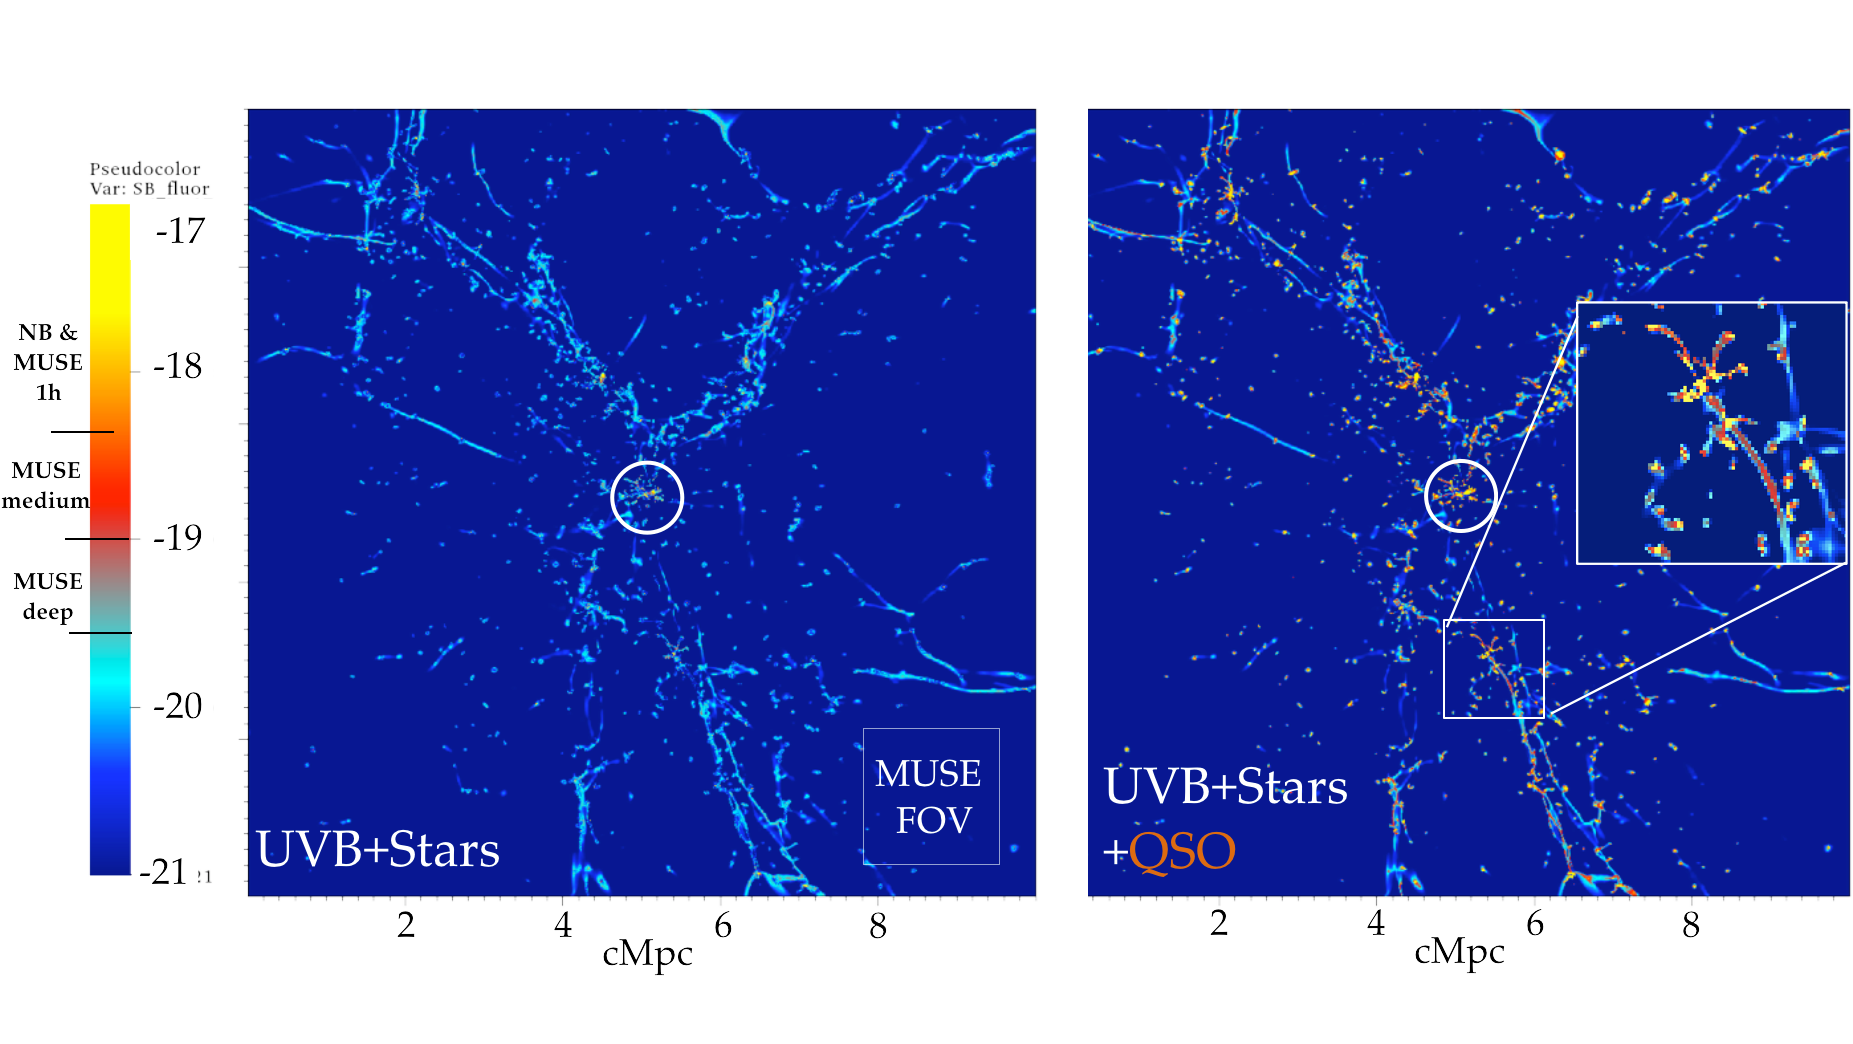
\includegraphics[height=15cm]{SC/Radamesh.png}
    \end{center}
  \end{minipage}

  \vspace{0.5cm}

  {\footnotesize \textit{[Cantalupo \& Porciani 2011, 2011MNRAS.411.1678C]}}
\end{section}